\documentclass{beamer}
\setbeamercovered{transparent}
\usepackage{listings}
\usepackage[T1]{fontenc}

\usetheme[pageofpages=of,% String used between the current page and the
                         % total page count.
          bullet=circle,% Use circles instead of squares for bullets.
          titleline=true,% Show a line below the frame title.
          titlepagelogo=opensuse,
          alternativetitlepage=true,% Use the fancy title page.
          ]{Torino}


% Define some stiles
\lstdefinestyle{mybash}{
  language=bash,
  basicstyle=\footnotesize\ttfamily,
  keywordstyle=\color{blue}\ttfamily,
  stringstyle=\color{red}\ttfamily,
  commentstyle=\color{green}\ttfamily,
  morecomment=[l][\color{magenta}]{\#}
}

\lstdefinestyle{myperl}{
  language=Perl,
  basicstyle=\footnotesize\ttfamily,
  keywordstyle=\color{blue}\ttfamily,
  stringstyle=\color{red}\ttfamily,
  commentstyle=\color{green}\ttfamily,
  morecomment=[l][\color{magenta}]{\#}
}


\setbeamerfont{title}{series=\bfseries,size=\LARGE}
\author{Alberto Planas <aplanas@suse.de>\newline {\small openSUSE Team}}
\title{openQA Workshop -- oSC14}
\subtitle{Learning how to make tests with openQA}


\AtBeginSection[]{
  \setbeamercolor{background canvas}{bg=chameleongreen3}
  \begin{frame}[plain]
    \begin{center}\begin{huge}\textcolor{white}{\secname}\end{huge}\end{center}
  \end{frame}
  \setbeamercolor{background canvas}{bg=}
}

\AtBeginSubsection[]{
  \setbeamercolor{background canvas}{bg=chameleongreen3}
  \begin{frame}[plain]
    \begin{center}\begin{huge}\textcolor{white}{\subsecname}\end{huge}\end{center}
  \end{frame}
  \setbeamercolor{background canvas}{bg=}
}


\begin{document}

\begin{frame}[t,plain]
  \titlepage
\end{frame}


\section{Introduction}
%
% Overview
%
\begin{frame}{Overview}
  With openQA we can test the installation process of a distribution.
  \begin{itemize}
  \item We provide the tests (Perl code)
  \item We provide the ISO image
  \item A worker will launch an instance of os-autoinst
  \item os-autoinst create the environment
    \begin{itemize}
    \item Environment variables
    \item HDD images
    \end{itemize}
  \item ... and run the tests
  \end{itemize}
\end{frame}

%
% Architecture
%
\begin{frame}{Architecture}
  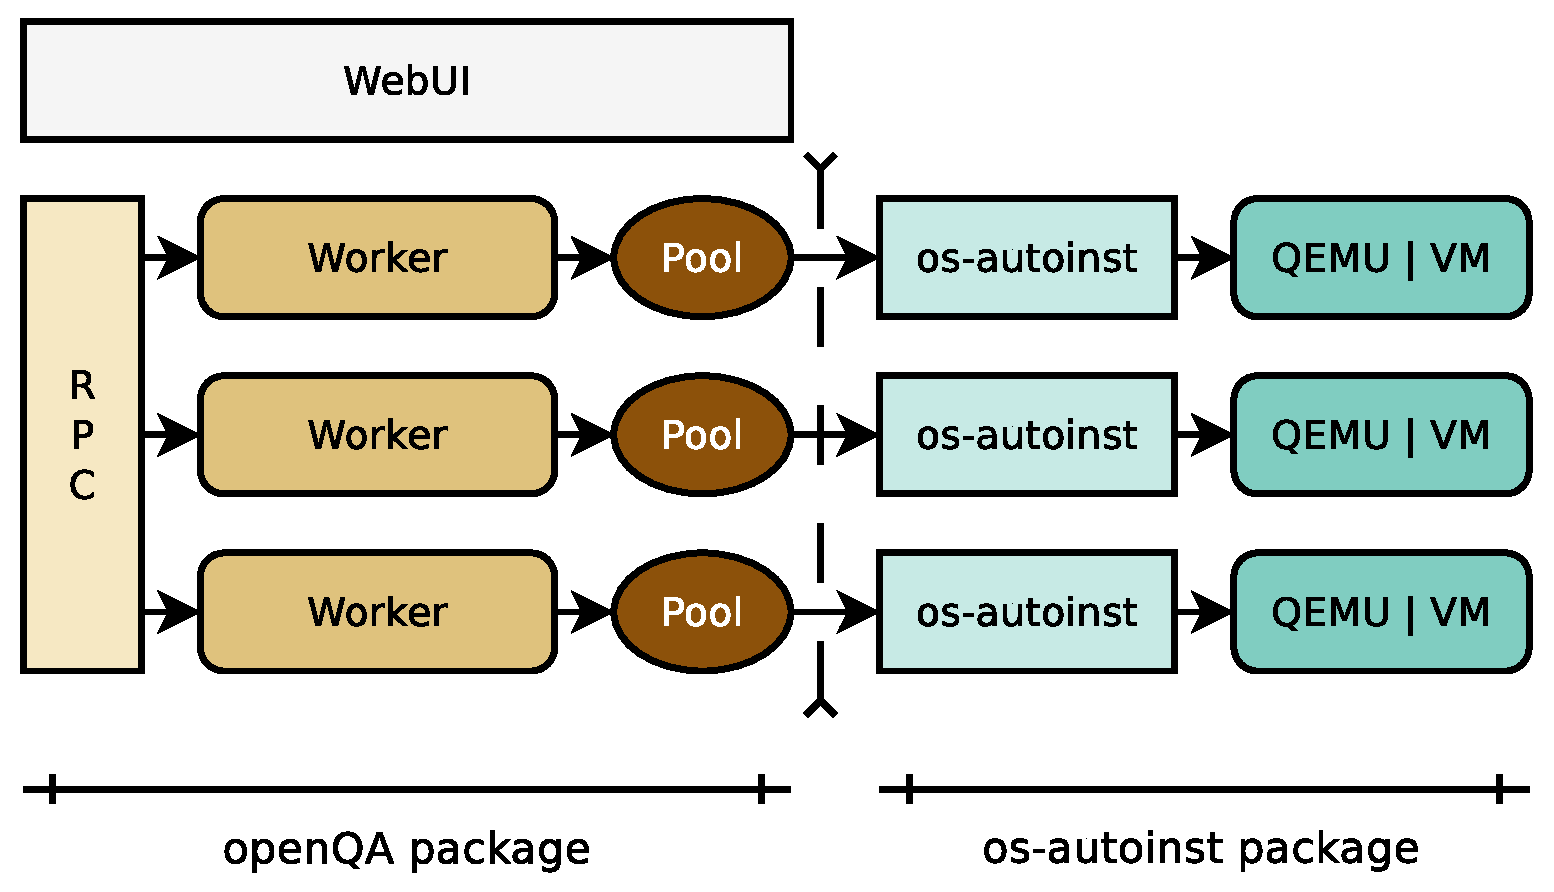
\includegraphics[height=5.8cm,width=10.3cm]{arch}
\end{frame}


\section{Installation}
%
% Installation
%
\begin{frame}[fragile]
  \frametitle{Installation}
  \begin{itemize}
  \item You can install from packages:
    \lstset{style=mybash}
    \begin{lstlisting}
zypper ar -f obs://devel:openQA/openSUSE_13.1 openQA
zypper ar -f obs://devel:openQA:13.1/openSUSE_13.1 openQA-perl-modules
zypper in openQA
# Start WebUI
systemctl start openqa-webui
    \end{lstlisting}
  \item More detailed instructions at \newline
    \url{https://github.com/os-autoinst/openQA}
  \end{itemize}
\end{frame}

%
% Test the Installation
%
\begin{frame}[fragile]
  \frametitle{Test the Installation}
  Download the ISO from
  \url{http://download.opensuse.org/factory/iso/}\newline
  and save to \texttt{/var/lib/openqa/factory/iso}

  Register the ISO ...
  \lstset{style=mybash}
  \begin{lstlisting}
/usr/share/openqa/script/client --host localhost:9526 \
  --key $KEY --secret $SECRET \
  isos post iso=openSUSE-13.1-DVD-x86_64-Build0091-Media.iso
  \end{lstlisting}

  ... launch the application ...
  \lstset{style=mybash}
  \begin{lstlisting}
    vi openqa.ini
    morbo script/openqa
  \end{lstlisting}

  ... and start the workers.
  \lstset{style=mybash}
  \begin{lstlisting}
    systemctl start openqa-worker.target
    # You can control every worker manually:
    # systemctl start openqa-worker@1.service
  \end{lstlisting}
\end{frame}

%
% Screen-shot of openQA
%
\begin{frame}{Screenshot}
  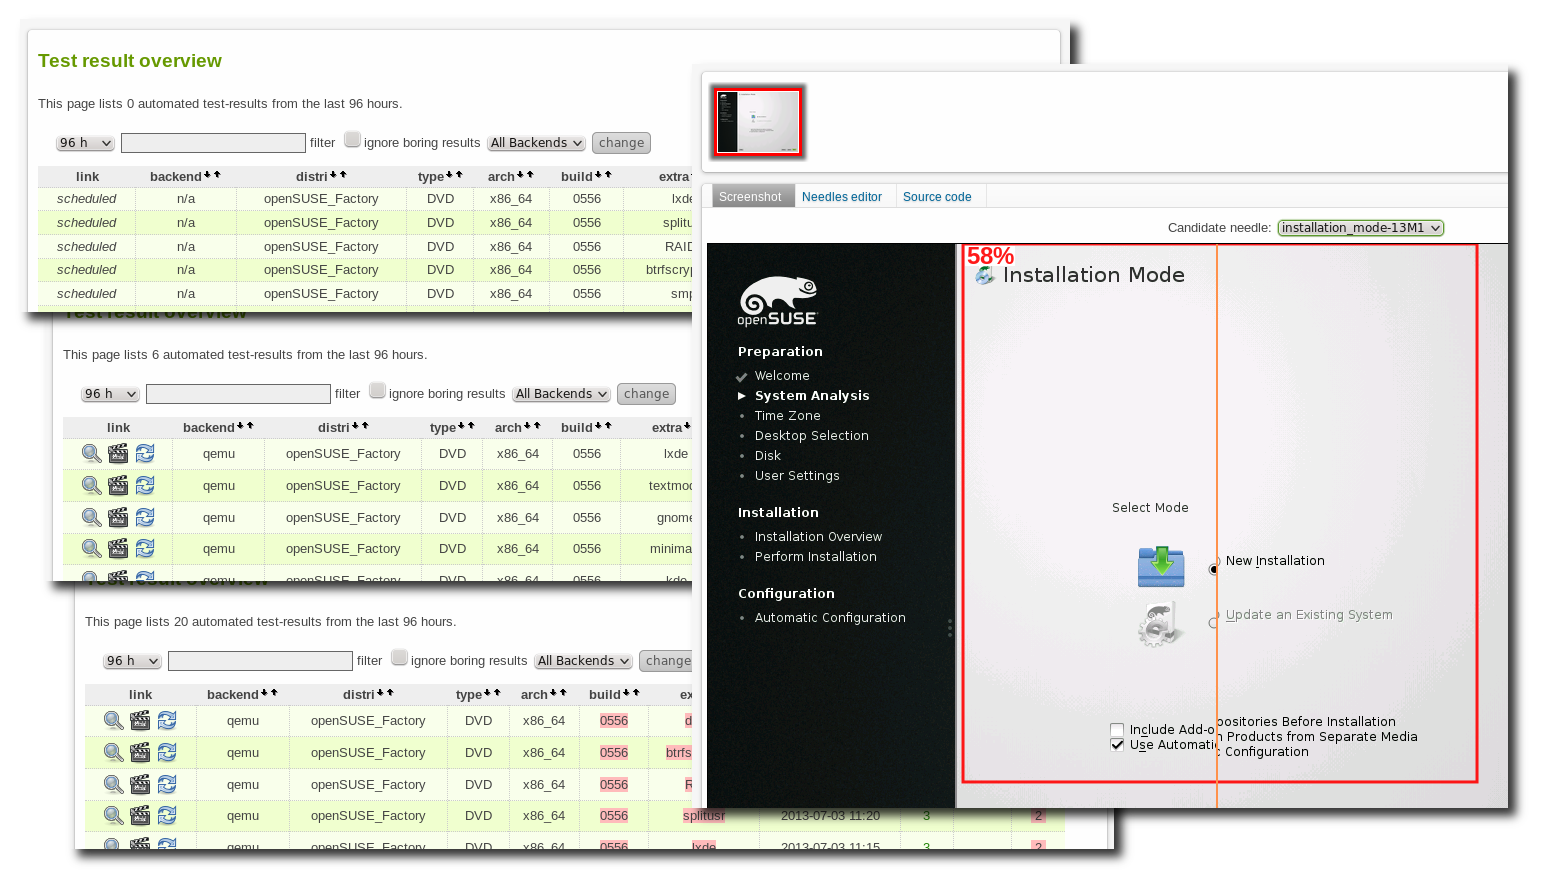
\includegraphics[height=6.2cm,width=10.88cm]{screenshot}
\end{frame}


\section{openQA Usage}
%
% Running a Test
%
\begin{frame}[fragile]
  \frametitle{Running a Test}
  \begin{itemize}
  \item Go to http://localhost:9526/
  \item Cancel all the test except KDE
  \item Launch in a terminal a new worker (if there is none via systemd)
    \lstset{style=mybash}
    \begin{lstlisting}
      ./script/worker --host localhost:9526 --instance 1 \
        --isotovideo=PATH_TO_isotovideo \
        --key $KEY --secret $SECRET
    \end{lstlisting}
  \item Refresh and see the test running
  \item You can connect via VNC
    \lstset{style=mybash}
    \begin{lstlisting}
      vncviewer localhost:91
    \end{lstlisting}
  \end{itemize}
\end{frame}

%
% Exercise 1
%
\begin{frame}{Exercise 1 -- Testing an ISO}
  \begin{enumerate}
  \item Use Build0575 to test a good ISO
  \item Register the ISO in the system
  \item Remove all jobs except the KDE one
  \item Launch only one worker
  \item Wait until fails!
  \end{enumerate}
\end{frame}

%
% Test Failed
%
\begin{frame}{Test Failed}
  So... the test failed. Let see what happen.
  \begin{itemize}
  \item Go to the result view
  \item Select the failed test
  \item Use the screenshot to check the image
  \item A real bug in Factory?
  \item If not, create a needle!
  \end{itemize}
\end{frame}

%
% The Needle
%
\begin{frame}[fragile]
  \frametitle{The Needle}
  A needle is a PNG image and a metadata in JSON
  \begin{columns}
    \begin{column}{0.45\textwidth}
    \lstset{style=mybash}
    \begin{lstlisting}
      {
        "area": [
          {
            "width": 514,
            "xpos": 255,
            "type": "match",
            "ypos": 0,
            "height": 538
          }
        ],
        "tags": [
          "inst-instmode"
        ]
      }
    \end{lstlisting}
    \end{column}

    \begin{column}{0.45\textwidth}
      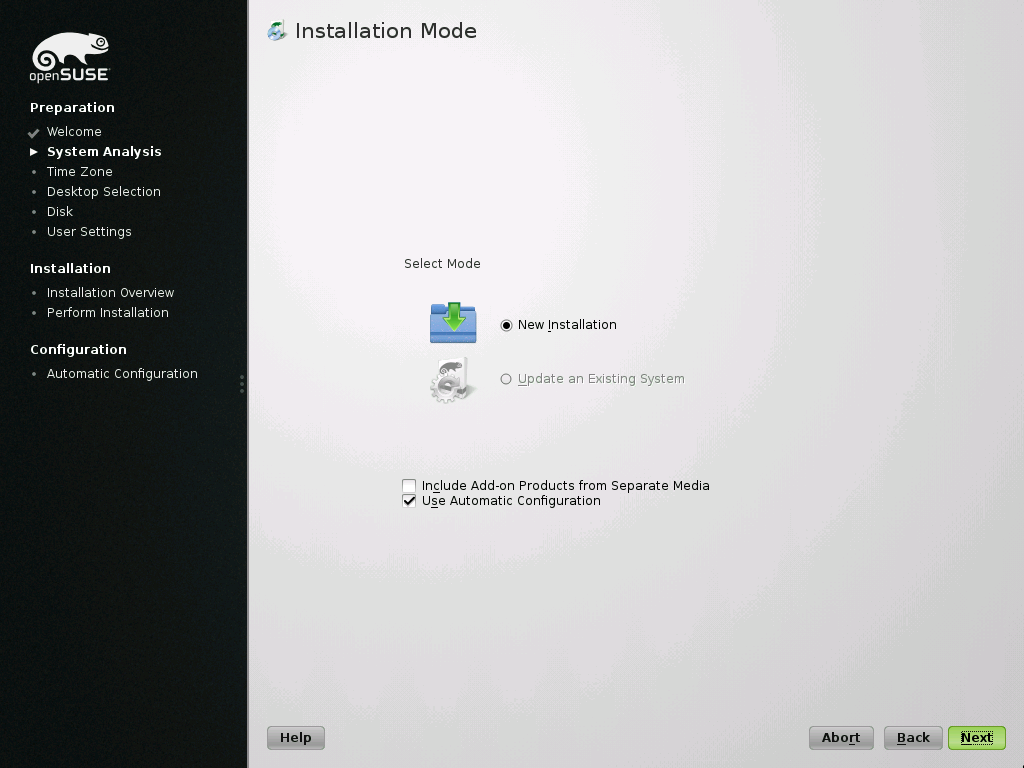
\includegraphics[height=4cm,width=5.33cm]{needle}
    \end{column}
  \end{columns}
\end{frame}

%
% Exercise 2
%
\begin{frame}{Exercise 2 -- Create a Needle}
  \begin{enumerate}
  \item Go to the result page
  \item Create a needle in the failing test
  \item Be careful with the TAGs!
  \item Relaunch the job and repeat the operation if needed
  \end{enumerate}
\end{frame}


\section{openQA API}
%
% Exercise 3
%
\begin{frame}{Exercise 3 -- Analyze a Test}
  \begin{enumerate}
  \item Use rpm -ql os-autoinst to find where are the tests
  \item Find the opensuse one and see the directories
  \item Read the ooffice test and figure out what is doing
  \end{enumerate}
\end{frame}

%
% API
%
\begin{frame}{Variables}
  Check the variables to see in what configuration are you
  \begin{itemize}
  \item DESKTOP = kde | gnome | lxde | minimalx ...
  \item USBBOOT | LIVETEST | NETBOOT
  \item BTRFS | ENCRYPT | LVM | RAIDLEVEL
  \item UEFI
  \end{itemize}
\end{frame}

\begin{frame}{API for Input}
  Sending events to the VM
  \begin{itemize}
  \item \texttt{sendkey "alt-n";} -- Send a keystroke
  \item \texttt{sendkey \$cmd\{"next"\};} -- Use the \texttt{\$cmd\{\}} map for shortcuts
  \item \texttt{sendautotype "string";} -- Send a set of keys
  \item \texttt{sendautotype("string", 3);}
  \end{itemize}
\end{frame}

\begin{frame}{API for Needles}
  Sending events to the VM
  \begin{itemize}
  \item \texttt{waitforneedle("tag", 1);} -- Assert for a needle that have this tag
  \item \texttt{checkneedle("tag", 1);} -- Return true is the needle is present
  \item \texttt{\$self->check\_screen;} -- Assert using a synthetic tag name (\texttt{test-\$testname-\$count})
  \item \texttt{\$self->take\_screenshot;} -- Do not assert. Journal for the test
  \end{itemize}
\end{frame}

%
% Directory layout
%
\begin{frame}{Directory layout}
  Two important directories:
  \begin{itemize}
  \item Tests: /usr/lib/os-autoinst/distri/opensuse
    \begin{itemize}
    \item Installation tests: inst.d
    \item Console tests: consoletest.d
    \item Application tests: x11test.d
    \end{itemize}
  \item Needles: /usr/lib/os-autoinst/distri/opensuse/needles
  \end{itemize}
\end{frame}

%
% Anatomy of a test
%
\begin{frame}[fragile]
  \frametitle{Anatomy of a Test I}
    \lstset{style=myperl}
    \begin{lstlisting}
      use base "basetest";
      use strict;
      use bmwqemu;

      # Determine, using the $ENV variables, if the
      # test can be selected for this configuration.
      sub is_applicable() {
      }

      # Main code of the test
      sub run() {
      }
    \end{lstlisting}
\end{frame}

\begin{frame}[fragile]
  \frametitle{Anatomy of a Test II}
    \lstset{style=myperl}
    \begin{lstlisting}
      # Return a map of flags to decide if the fail
      # of this test is important, or to decide a
      # rollback of the VM status.
      sub test_flags() {
      }

      1;
    \end{lstlisting}
\end{frame}

\begin{frame}{Test Flags}
  With the tests flags we control the behavior of the test if it fails.
  \begin{itemize}
  \item \texttt{\{ 'fatal'=>1 \}} -- If fails, the test suite fails
  \item \texttt{\{ 'important'=>1 \}} -- If fails, the overall state fails. Factory is broken
  \item \texttt{\{ 'milestone'=>1 \}} -- If ok, generate a new 'lastgood' snapshot
  \item \texttt{\{ \}} -- If fails, recover the 'lastgood' snapshot and continue to the next test
  \end{itemize}
\end{frame}


%
% Exercise 4
%
\begin{frame}{Exercise 4 -- A test for Okular}
  \begin{enumerate}
  \item Create a test for okular
  \item ... or evince 
  \end{enumerate}
\end{frame}


\begin{frame}[fragile]
  \frametitle{A test for Okular}
  This is an application test
  \lstset{style=myperl}
  \begin{lstlisting}
    use base "basetest";
    use strict;
    use bmwqemu;

    sub is_applicable() {
      return $ENV{DESKTOP} eq "kde";
    }

    sub run() {
      my $self=shift;
      sendkey "alt-f2"; sendautotype "okular";
      sendkey "ret"; waitforneedle("okular", 5);
      sendkey "alt-f4"; sendkey "ret";
    }

    1;
  \end{lstlisting}
\end{frame}

\begin{frame}[fragile]
  \frametitle{A test for Okular -- Sleeping}
  But is not working!! -- We need to sleep.
  \lstset{style=myperl}
  \begin{lstlisting}
    [...]
    sub run() {
      my $self=shift;
      sendkey "alt-f2"; sleep 2;
      sendautotype "okular"; sleep 2;
      sendkey "ret"; sleep 2;
      waitforneedle("okular", 5);
      sendkey "alt-f4"; sleep 2;
      sendkey "ret";
    }
    [...]
  \end{lstlisting}
\end{frame}

\begin{frame}{API to Run Programs}
  We can hide the sleep command... a bit.
  \begin{itemize}
  \item \texttt{script\_run("program");} -- Run the program from a terminal
  \item \texttt{script\_sudo("program");} -- Run the program as root
  \item \texttt{x11\_start\_program("program");} -- You have implemented that
  \end{itemize}
\end{frame}

%
% Exercise 5
%
\begin{frame}{Exercise 5 -- The sudo Case}
  \begin{enumerate}
  \item From time to time we want to run a program with sudo
  \item sudo can ask for a password, sometimes
  \item Figure out how to resolve this problem with the current API
  \item If you are out of ideas, find the implementation and try to understand it
  \end{enumerate}
\end{frame}


\begin{frame}[fragile]
  \frametitle{The sudo Case}
  With checkneedle we can add state into a test. This state is needed
  to check when the terminal is asking for the root password.
  \lstset{style=myperl}
  \begin{lstlisting}
    sendautotype("sudo ls\n");
    if (checkneedle("sudo-prompt", 2)) {
      sendautotype("p4ssw0rd");
      sendkey "ret";
    }
  \end{lstlisting}
\end{frame}

\begin{frame}[fragile]
  \frametitle{A Complex Case}
  How to resolve when a dialog box appears during the installation process?
  \lstset{style=myperl}
  \begin{lstlisting}
    my @tags = (@{needle::tags("good-needle")},
                @{needle::tags("bad-needle")});
    my $err = 0;
    while (1) {
      my $ret = waitforneedle(\@tags, 200);
      last if $ret->{needle}->has_tag("good-needle");
      $self->take_screenshot;
      sendkey "ret";
      $err = 1;
    }
    mydie if $err;
  \end{lstlisting}
\end{frame}


\begin{frame}{Advanced API}
  \begin{itemize}
  \item \texttt{qemusend "command";} -- Send QEMU commands directly
  \item \texttt{makesnapshot "name";} -- Create a VM snapshot
  \item \texttt{loadsnapshot "name";} -- Recover a VM snapshot
  \item \texttt{mouse\_[move|set|click](x, y);} -- Control the mouse
  \item \texttt{mouse\_hide;} -- Hide the mouse
  \item \texttt{waitserial "regexp";} -- Result 1 if found in the serial port
  \end{itemize}
\end{frame}


\section{Endnote}

\begin{frame}{Suse is hiring}
  \begin{figure}
    
\includegraphics[width= 0.8\linewidth]{suse_hiring.png}
  \end{figure}
\end{frame}

\begin{frame}{Thanks}
  \begin{center}
    Thank you for your attention.
  \end{center}
\end{frame}

\end{document}
